This report details my implementation of the stochastic simulation library using the Doob-Gillespie algorithm.
Both the report and library were implemented for the Selected Topics in Programming course at Aalborg University, 2023.

Along with this report is attached an archive containing the library files, including \texttt{CMakeLists.txt} files, so that it can be compiled.
These files can also be found on this \href{https://github.com/chhoumann/selected_topics_in_programming_8_semester/tree/master/exam_assignment}{GitHub repository}\footnote{\url{https://github.com/chhoumann/selected_topics_in_programming_8_semester/tree/master/exam_assignment}}.

\section{Project setup}
The project uses a few packages to implement the stochastic simulation library.
For testing, \texttt{googletest} is used. This is fetched automatically via \texttt{test/CMakeLists.txt}.

Graphviz is used for creating reaction network graphs. It is, on the other hand, not fetched automatically.
Since I am using Ubuntu via WSL2, I installed Graphviz for development via \texttt{sudo apt install libgraphviz-dev}.

The project also heavily relies on the course-provided plotting library, which uses qt5charts.
This can be installed via \texttt{sudo apt install libqt5charts5-dev}. The plotting library has been modified to accomodate new uses.

The \texttt{CMakeLists.txt} files show how the project is compiled.
The commands used to compile the project can be seen in code snippet \ref{lst:buildScript}. 
Do note that I used CLion to compile the project, but have successfully used the script below to compile the project.

\begin{lstlisting}[language=bash, caption={Bash script for building project}, label={lst:buildScript}, style=colorBash]
#!/bin/bash

# create a build directory if it doesn't exist
mkdir -p build
cd build

# compile with Debug configuration
cmake .. -DCMAKE_BUILD_TYPE=Debug

# compile with Release configuration (comment out the previous line if you want to compile in Release mode)
# cmake .. -DCMAKE_BUILD_TYPE=Release

# build the project
make
\end{lstlisting}

\subsection{Project structure}
\dirtree{%
.1 /.
.2 CMakeLists.txt.
.2 src.
.3 CMakeLists.txt.
.3 examples.
.4 circadian\_oscillator.cpp.
.4 examples.h.
.4 seihr.cpp.
.4 simple.cpp.
.3 exercises.
.4 benchmark.cpp.
.4 benchmark.h.
.4 make\_graphs.cpp.
.4 make\_graphs.h.
.4 peak\_avg\_seihr.cpp.
.4 peak\_avg\_seihr.h.
.3 graph\_generator.cpp.
.3 graph\_generator.h.
.3 main.cpp.
.3 monitor.
.4 monitor.h.
.4 species\_peak\_monitor.cpp.
.4 species\_peak\_monitor.h.
.4 species\_trajectory\_monitor.cpp.
.4 species\_trajectory\_monitor.h.
.3 parallel\_simulator.h.
.3 plot.
.4 plot.cpp.
.4 plot.hpp.
.3 reaction\_rule\_printer.cpp.
.3 stochastic\_simulator.cpp.
.3 stochastic\_simulator.h.
.3 symbol\_table.cpp.
.3 thread\_pool.h.
.3 types.cpp.
.3 types.h.
.2 tests.
.3 CMakeLists.txt.
.3 main.cpp.
}

\section{Demonstration}
Each of these were run after building the library in release mode.

\subsection{Pretty-printing in human-readable format}
\subsubsection{SEIHR}
\begin{verbatim}
S + I -> E + I (rate: 7.74194e-06)
E -> I (rate: 0.196078)
I -> R (rate: 0.322581)
I -> H (rate: 0.000290061)
H -> R (rate: 0.0988142)
\end{verbatim}

\subsubsection{Circadian Oscillator}
\begin{verbatim}
A + DA -> D_A (rate: 1)
D_A -> DA + A (rate: 50)
A + DR -> D_R (rate: 1)
D_R -> DR + A (rate: 100)
D_A -> MA + D_A (rate: 500)
DA -> MA + DA (rate: 50)
D_R -> MR + D_R (rate: 50)
DR -> MR + DR (rate: 0.01)
MA -> MA + A (rate: 50)
MR -> MR + R (rate: 5)
A + R -> C (rate: 2)
C -> R (rate: 1)
A -> environment (rate: 1)
R -> environment (rate: 0.2)
MA -> environment (rate: 10)
MR -> environment (rate: 0.5)
\end{verbatim}

\subsubsection{Simple}
\begin{verbatim}
A + C -> B + C (rate: 0.001)
\end{verbatim}

\subsection{Reaction network graphs}
Figure~\ref{fig:graphs} shows the reaction network graphs.
The graphs were generated using the \texttt{graphviz} library.
Subsection \ref{subsection:graph_generator} shows how the graphs are created.

\begin{figure}[H]
\centering
\begin{subfigure}{.3\textwidth}
  \centering
  \includegraphics[width=.9\linewidth]{images/circadian\_graph.png}
  \caption{Circadian Graph}
  \label{fig:circadian}
\end{subfigure}%
\begin{subfigure}{.3\textwidth}
  \centering
  \includegraphics[width=.9\linewidth]{images/simple\_graph.png}
  \caption{Simple Graph}
  \label{fig:simple}
\end{subfigure}
\begin{subfigure}{.3\textwidth}
  \centering
  \includegraphics[width=.9\linewidth]{images/seihr\_graph.png}
  \caption{SEIHR Graph}
  \label{fig:seihr}
\end{subfigure}
\caption{Reaction graphs over various systems}
\label{fig:graphs}
\end{figure}

\subsection{Simulations}
The following figures show simulations run on the systems shown in Figure~\ref{fig:graphs}.
These graphs show the evolution of the agents of various species within the system over time, as reactions occur.

\subsubsection{Simple system}
Figure~\ref{fig:simple_sim} shows a simple system simulation.
The implementation of the system is shown in section \ref{subsection:simple}, and the plot implementation is shown in section \ref{subsection:main}, in the \texttt{plot\_simple} function.

\begin{figure}[H]
\centering
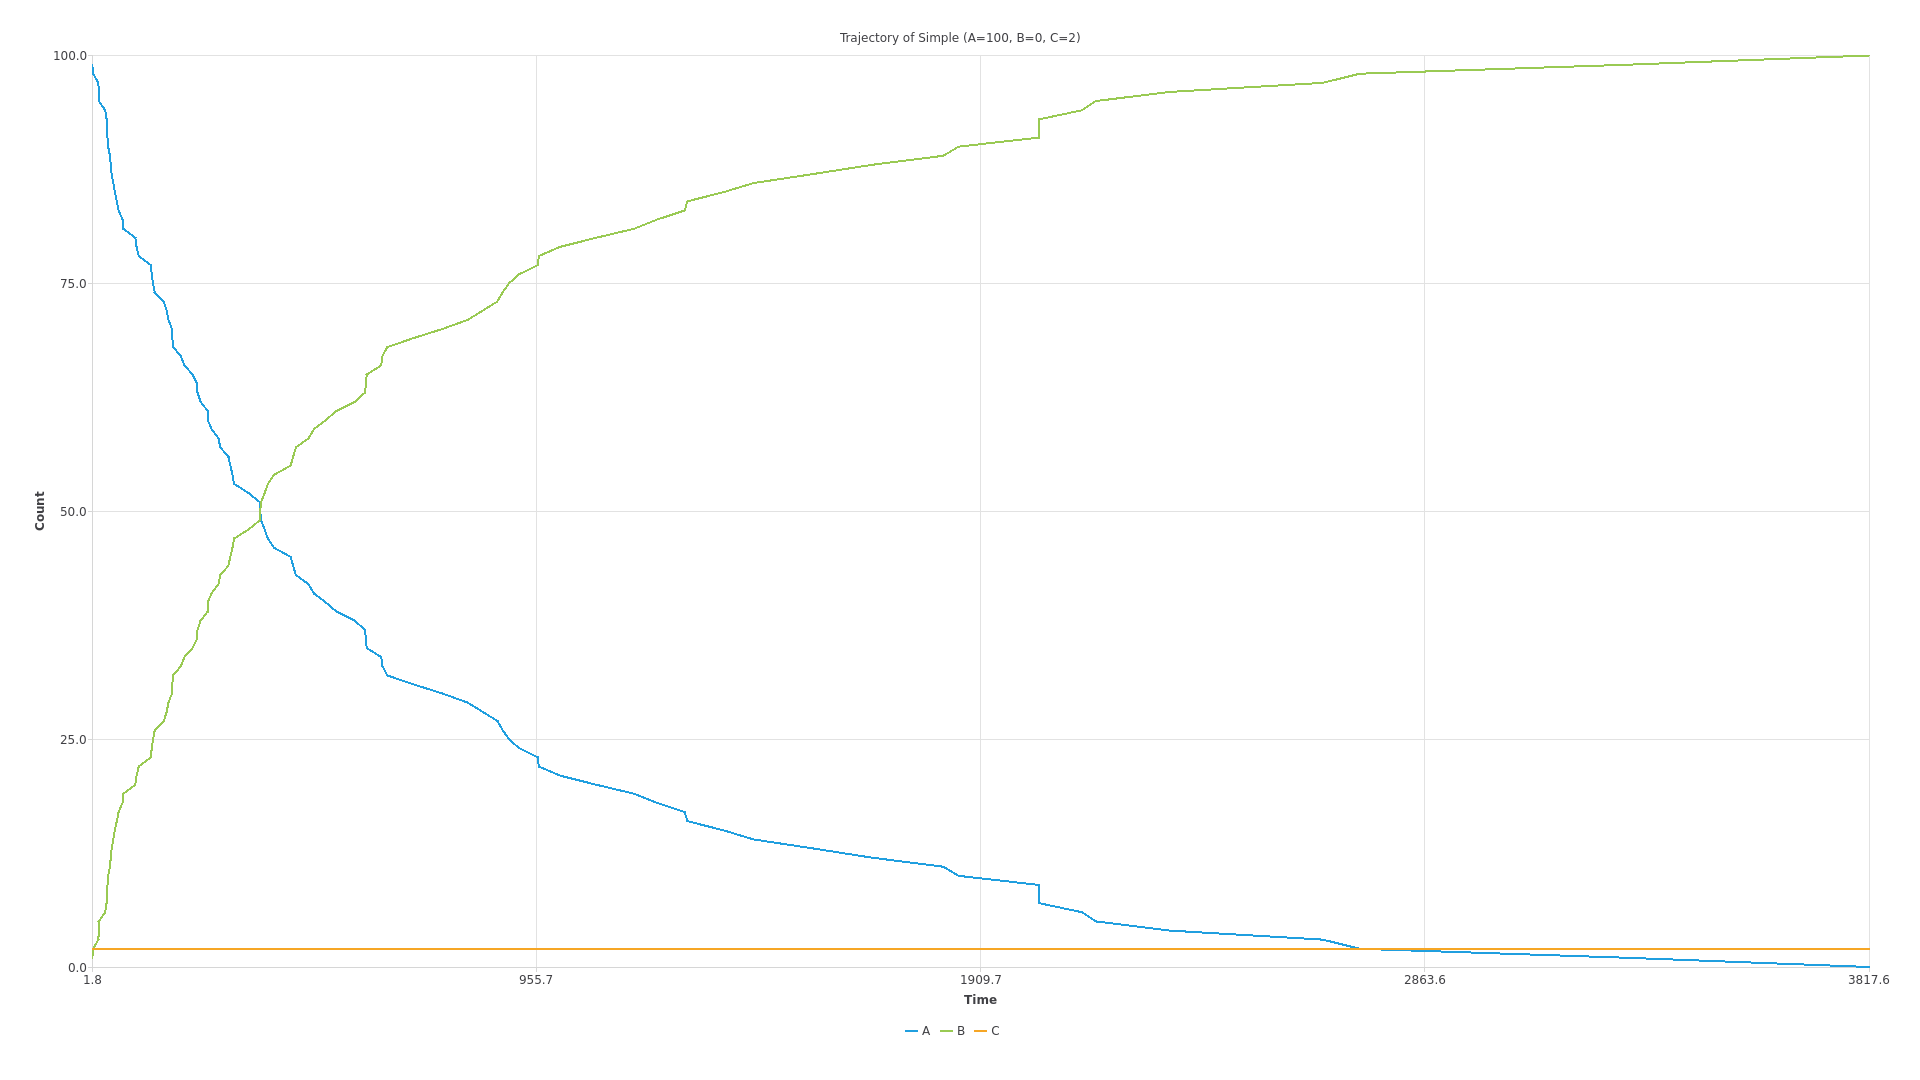
\includegraphics[width=1\textwidth,height=\textheight,keepaspectratio]{images/simple.png}
\caption{Simple system simulation, given by A=100, B=0, C=2. Simulation end time set to $100.000$, but ends prior to that as no further reactions were possible.}
\label{fig:simple_sim}
\end{figure}

\subsubsection{Circadian Oscillator}
Figure~\ref{fig:circadian_sim} shows a circadian system simulation.
The implementation of the system is shown in section \ref{subsection:circadian_oscillator}, and the plot implementation is shown in section \ref{subsection:main}, in the \texttt{plot\_circadian} function.

\begin{figure}[H]
\centering
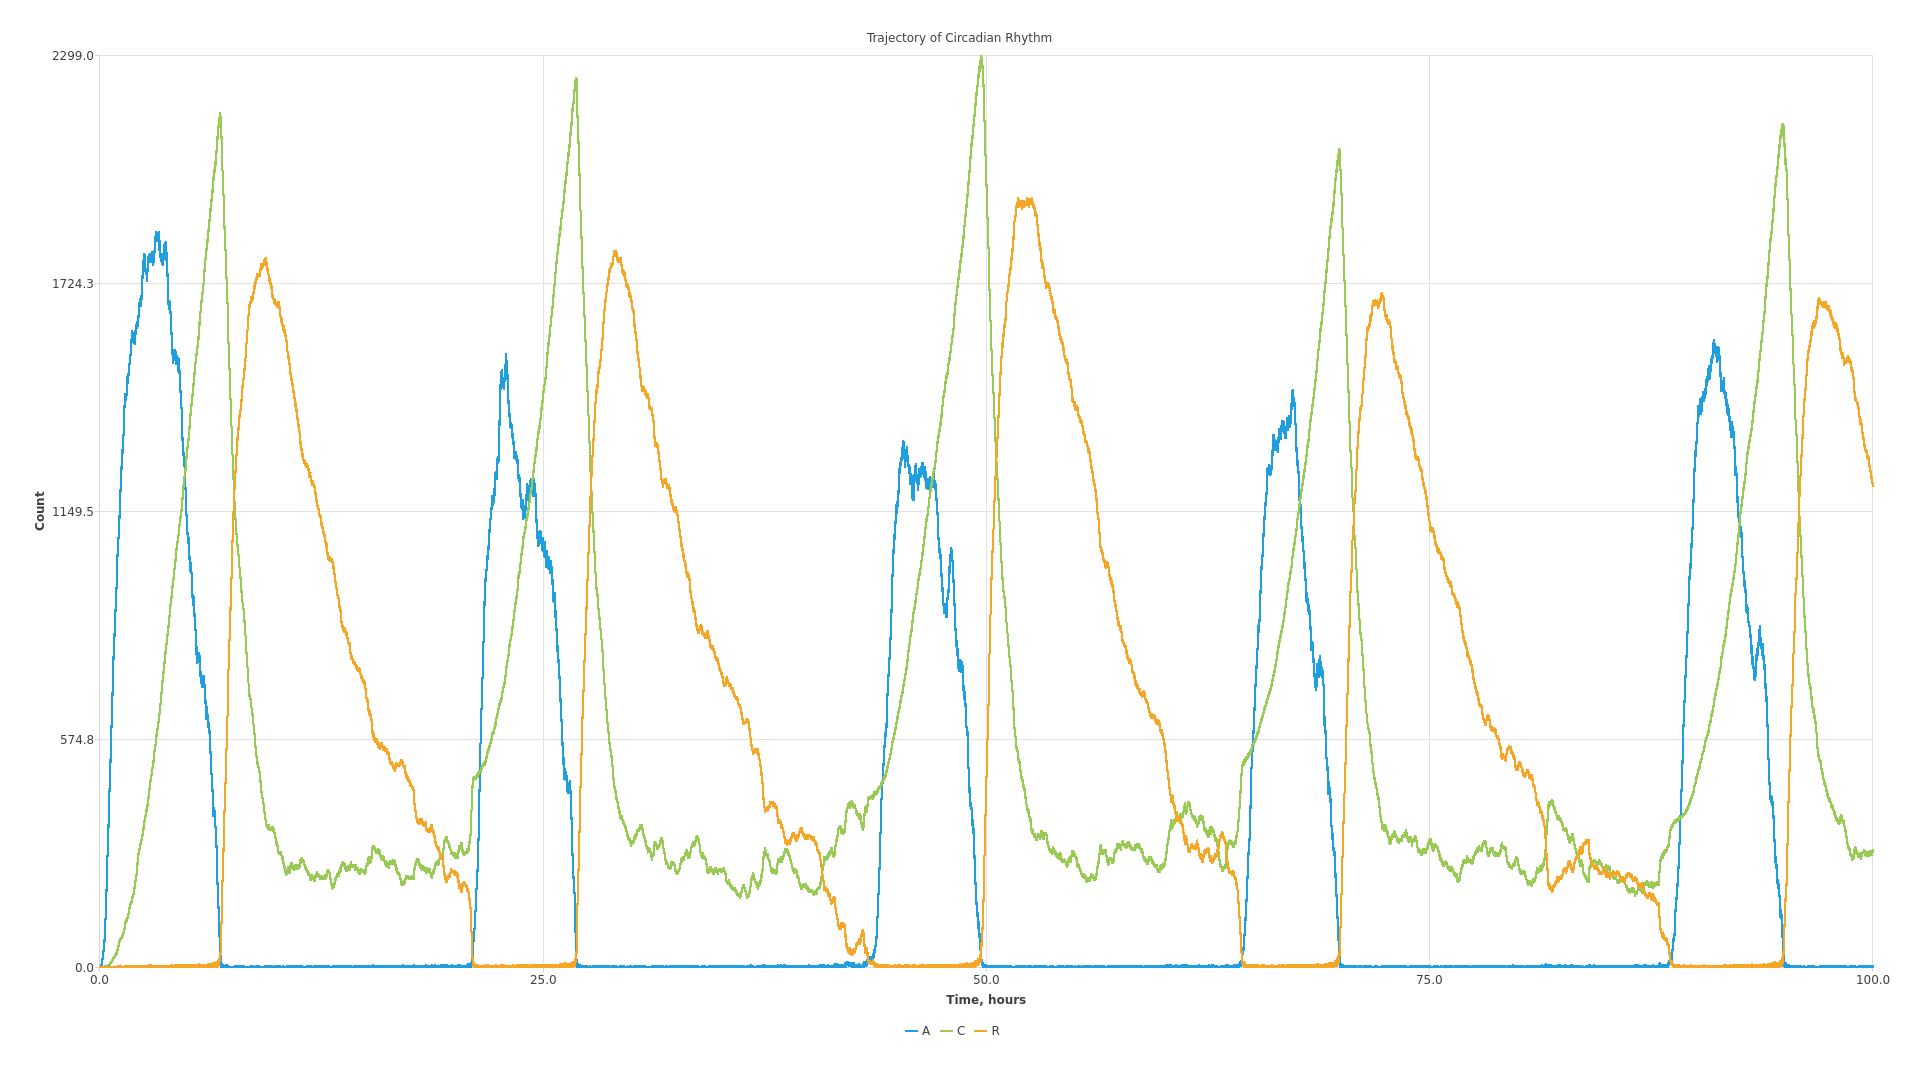
\includegraphics[width=1\textwidth,height=\textheight,keepaspectratio]{images/circadian.png}
\caption{Circadian system simulation. Simulation end time set to $100$. Graph shows evolution of agents of \textit{C}, \textit{A}, and \textit{R} over time.}
\label{fig:circadian_sim}
\end{figure}

\subsubsection{SEIHR}
Figure~\ref{fig:seihr_sim} shows a SEIHR system simulation.
The implementation of the system is shown in section \ref{subsection:seihr}, and the plot implementation is shown in section \ref{subsection:main}, in the \texttt{plot\_seihr} function.

\begin{figure}[H]
\centering
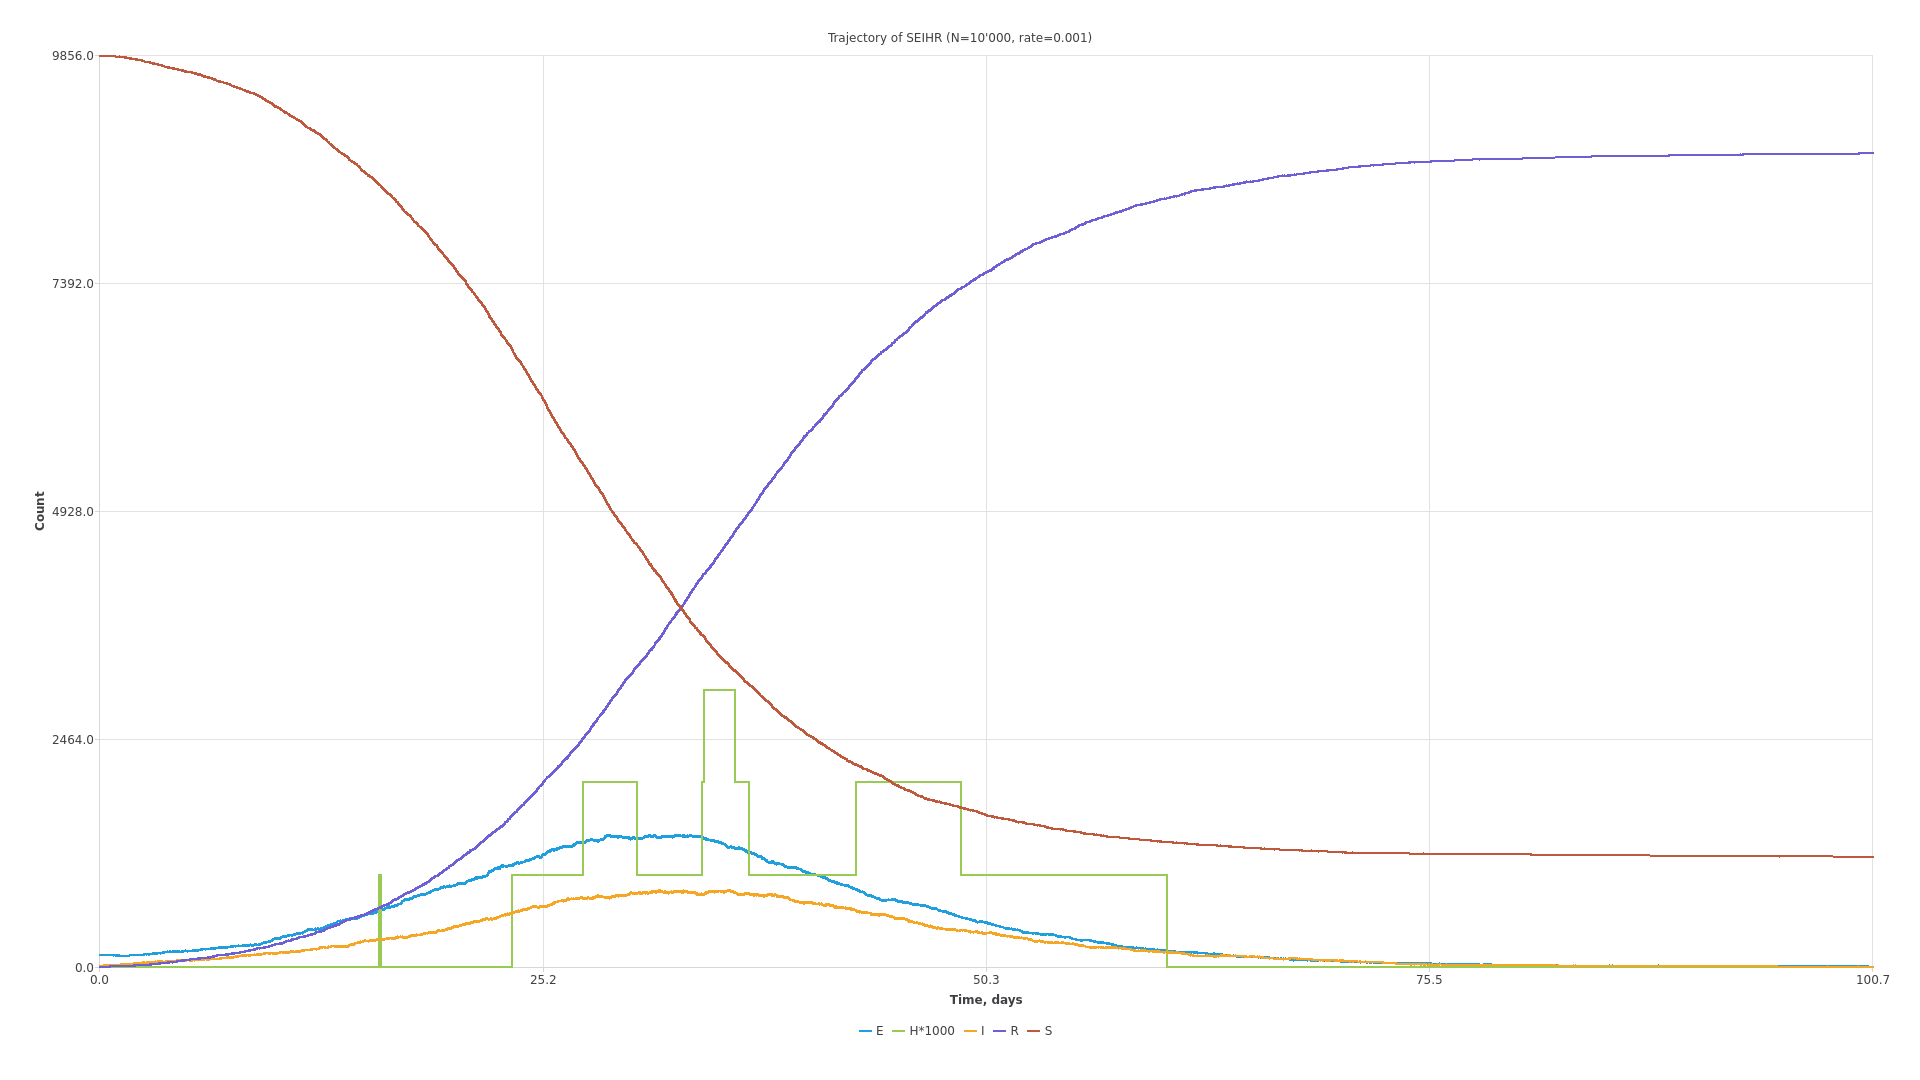
\includegraphics[width=1\textwidth,height=\textheight,keepaspectratio]{images/seihr.png}
\caption{SEIHR system simulation. For this simulation, $N=10.000$. Simulation end time set to $100$. \textit{H}ospitalized agent quantities are multiplied by $1000$ to make them visible on the graph.}
\label{fig:seihr_sim}
\end{figure}

\subsection{Peak hospitalized via SEIHR simulations}
The following numbers show the average and peak number of hospitalizations over time, averaged over $100$ simulations.
The peak number of hospitalizations is the maximum number of hospitalizations at any given time.

The implementation of the system is shown in section \ref{subsection:seihr}, and the calculation implementation is shown in section \ref{subsection:peak_avg_seihr}.

\begin{table}[ht]
\centering
\begin{tabular}{|l|c|c|}
\hline
\textbf{Population ($N$)} & \textbf{Avg Peak Hospitalized} & \textbf{Max Peak Hospitalized} \\
\hline
North Jutland ($589.755$) & 126.96 & 149 \\
\hline
Denmark ($5.882.763$) & 1206.95 & 1278 \\
\hline
\end{tabular}
\caption{Average and maximum peak of hospitalized cases over $100$ simulations for different population sizes}
\end{table}

\subsection{Benchmarks}
The following table shows benchmark results by benchmarking parallel and sequential simulations of the SEIHR system.
The implementation of the system is shown in section \ref{subsection:seihr}, and the benchmark implementation is shown in section \ref{subsection:benchmark}.

The benchmarks were run on a computer with an Intel(R) Core(TM) i7-8700K CPU, which has 6 cores \& 12 logical processors.

The SEIHR system was given a population of $N=10.000$ and the simulation end time set to $100$.
An empty state monitor was used to avoid any overhead from the state monitor.

Prior to benchmarking, the computer was warmed up via a short warming-up process of running the simulation $10$ times with the first benchmark configuration (1 thread, 10 simulations).
Each configuration was run 5 times and then the results for those five runs were averaged.

Due to the system used to benchmark the simulations, I chose concurrency levels of $1$, $6$, $12$, and $18$.
I expect that, due to the amount of processors, parallel simulation with 12 threads is the fastest configuration.
This is because fewer threads would not utilize the system adequately, and more threads would simply lead to additional, unnecessary overhead.

The benchmark results are shown in Table~\ref{tab:benchmark_results}.
The results show that the parallel simulation is faster than the sequential simulation, and that, as expected, 12 threads is the fastest configuration.


\begin{table}[htbp]
\centering
\begin{tabular}{|l|c|c|c|c|c|c|c|c|}
\hline
 & \multicolumn{2}{c|}{CL 1} & \multicolumn{2}{c|}{CL 6} & \multicolumn{2}{c|}{CL 12} & \multicolumn{2}{c|}{CL 18} \\
\hline
Simulations & Avg Time & Total Time & Avg Time & Total Time & Avg Time & Total Time & Avg Time & Total Time \\
\hline
$10$ & $21$.$18$ ms & $1$ s & $17$.$72$ ms & $0$ s & $22$.$34$ ms & $0$ s & $26$.$15$ ms & $0$ s \\
\hline
$100$ & $17$.$56$ ms & $8$ s & $17$.$81$ ms & $1$ s & $26$.$26$ ms & $1$ s & $42$.$44$ ms & $1$ s \\
\hline
$1000$ & $14$.$18$ ms & $71$ s & $17$.$56$ ms & $14$ s & $26$.$73$ ms & $11$ s & $42$.$00$ ms & $13$ s \\
\hline
$10000$ & $14$.$14$ ms & $711$ s & $17$.$73$ ms & $148$ s & $30$.$25$ ms & $126$ s & $40$.$85$ ms & $130$ s \\
\hline
\end{tabular}
\caption{Benchmark results showing average and total runtime for each simulation under different concurrency levels (CL)}
\label{tab:benchmark_results}
\end{table}

The following figures illustrate the benchmark results from Table~\ref{tab:benchmark_results} clearly.
As we can see in Figure~\ref{fig:avg_sim_benchmark_results}, task times grow with increasing concurrency levels.
This is to be expected, as the system is under greater load, so the time it takes to complete a task increases.
However, as we can see in Figure~\ref{fig:total_sim_benchmark_results}, the total time decreases with increasing concurrency levels.

\begin{figure}[H]
\centering
\includegraphics[width=1\textwidth,height=\textheight,keepaspectratio]{images/avg\_sim\_benchmark\_results.png}
\caption{Benchmark results showing average runtime for each simulation under different concurrency levels (CL).}
\label{fig:avg_sim_benchmark_results}
\end{figure}

\begin{figure}[H]
\centering
\includegraphics[width=1\textwidth,height=\textheight,keepaspectratio]{images/total\_sim\_benchmark\_results.png}
\caption{Benchmark results showing total runtime for each simulation under different concurrency levels (CL).}
\label{fig:total_sim_benchmark_results}
\end{figure}



\newpage

\section{Source code}
% Main CMakeLists.txt file
\subsection{CMakeLists.txt}
\lstinputlisting[style=colorC++,caption={CMakeLists.txt}]{../../CMakeLists.txt}

% src directory
\newpage
\subsection{src}
\subsubsection{src/CMakeLists.txt}
\lstinputlisting[style=colorC++,caption={src/CMakeLists.txt}]{../../src/CMakeLists.txt}
\newpage
\subsubsection{src/main.cpp}\label{subsection:main}
\lstinputlisting[style=colorC++,caption={src/main.cpp}]{../../src/main.cpp}
\newpage
\subsubsection{src/graph\_generator.cpp}\label{subsection:graph_generator}
\lstinputlisting[style=colorC++,caption={src/graph\_generator.cpp}]{../../src/graph\_generator.cpp}
\newpage
\subsubsection{src/graph\_generator.h}
\lstinputlisting[style=colorC++,caption={src/graph\_generator.h}]{../../src/graph\_generator.h}
\newpage
\subsubsection{src/parallel\_simulator.h}
\lstinputlisting[style=colorC++,caption={src/parallel\_simulator.h}]{../../src/parallel\_simulator.h}
\newpage
\subsubsection{src/stochastic\_simulator.cpp}
\lstinputlisting[style=colorC++,caption={src/stochastic\_simulator.cpp}]{../../src/stochastic\_simulator.cpp}
\newpage
\subsubsection{src/stochastic\_simulator.h}
\lstinputlisting[style=colorC++,caption={src/stochastic\_simulator.h}]{../../src/stochastic\_simulator.h}
\newpage
\subsubsection{src/symbol\_table.cpp}
\lstinputlisting[style=colorC++,caption={src/symbol\_table.cpp}]{../../src/symbol\_table.cpp}
\newpage
\subsubsection{src/thread\_pool.h}
\lstinputlisting[style=colorC++,caption={src/thread\_pool.h}]{../../src/thread\_pool.h}
\newpage
\subsubsection{src/types.cpp}
\lstinputlisting[style=colorC++,caption={src/types.cpp}]{../../src/types.cpp}
\newpage
\subsubsection{src/types.h}
\lstinputlisting[style=colorC++,caption={src/types.h}]{../../src/types.h}

% src/examples directory
\newpage
\subsection{src/examples}
\subsubsection{src/examples/circadian\_oscillator.cpp}\label{subsection:circadian_oscillator}
\lstinputlisting[style=colorC++,caption={src/examples/circadian\_oscillator.cpp}]{../../src/examples/circadian\_oscillator.cpp}
\newpage
\subsubsection{src/examples/examples.h}
\lstinputlisting[style=colorC++,caption={src/examples/examples.h}]{../../src/examples/examples.h}
\newpage
\subsubsection{src/examples/seihr.cpp}\label{subsection:seihr}
\lstinputlisting[style=colorC++,caption={src/examples/seihr.cpp}]{../../src/examples/seihr.cpp}
\newpage
\subsubsection{src/examples/simple.cpp}\label{subsection:simple}
\lstinputlisting[style=colorC++,caption={src/examples/simple.cpp}]{../../src/examples/simple.cpp}

% src/exercises directory
\newpage
\subsection{src/exercises}
\subsubsection{src/exercises/benchmark.cpp}\label{subsection:benchmark}
\lstinputlisting[style=colorC++,caption={src/exercises/benchmark.cpp}]{../../src/exercises/benchmark.cpp}
\newpage
\subsubsection{src/exercises/benchmark.h}
\lstinputlisting[style=colorC++,caption={src/exercises/benchmark.h}]{../../src/exercises/benchmark.h}
\newpage
\subsubsection{src/exercises/make\_graphs.cpp}
\lstinputlisting[style=colorC++,caption={src/exercises/make\_graphs.cpp}]{../../src/exercises/make\_graphs.cpp}
\newpage
\subsubsection{src/exercises/make\_graphs.h}
\lstinputlisting[style=colorC++,caption={src/exercises/make\_graphs.h}]{../../src/exercises/make\_graphs.h}
\newpage
\subsubsection{src/exercises/peak\_avg\_seihr.cpp}\label{subsection:peak_avg_seihr}
\lstinputlisting[style=colorC++,caption={src/exercises/peak\_avg\_seihr.cpp}]{../../src/exercises/peak\_avg\_seihr.cpp}
\newpage
\subsubsection{src/exercises/peak\_avg\_seihr.h}
\lstinputlisting[style=colorC++,caption={src/exercises/peak\_avg\_seihr.h}]{../../src/exercises/peak\_avg\_seihr.h}

% src/monitor directory
\newpage
\subsection{src/monitor}
\subsubsection{src/monitor/monitor.cpp}
\lstinputlisting[style=colorC++,caption={src/monitor/monitor.h}]{../../src/monitor/monitor.h}
\newpage
\subsubsection{src/monitor/species\_peak\_monitor.cpp}
\lstinputlisting[style=colorC++,caption={src/monitor/species\_peak\_monitor.cpp}]{../../src/monitor/species\_peak\_monitor.cpp}
\newpage
\subsubsection{src/monitor/species\_peak\_monitor.h}
\lstinputlisting[style=colorC++,caption={src/monitor/species\_peak\_monitor.h}]{../../src/monitor/species\_peak\_monitor.h}
\newpage
\subsubsection{src/monitor/species\_trajectory\_monitor.cpp}
\lstinputlisting[style=colorC++,caption={src/monitor/species\_trajectory\_monitor.cpp}]{../../src/monitor/species\_trajectory\_monitor.cpp}
\newpage
\subsubsection{src/monitor/species\_trajectory\_monitor.h}
\lstinputlisting[style=colorC++,caption={src/monitor/species\_trajectory\_monitor.h}]{../../src/monitor/species\_trajectory\_monitor.h}

% src/plot directory
\newpage
\subsection{src/plot}
\subsubsection{src/plot/plot.cpp}
\lstinputlisting[style=colorC++,caption={src/plot/plot.cpp}]{../../src/plot/plot.cpp}
\newpage
\subsubsection{src/plot/plot.hpp}
\lstinputlisting[style=colorC++,caption={src/plot/plot.hpp}]{../../src/plot/plot.hpp}

% tests directory
\newpage
\subsection{tests}
\subsubsection{tests/CMakeLists.txt}
\lstinputlisting[style=colorC++,caption={tests/CMakeLists.txt}]{../../tests/CMakeLists.txt}
\newpage
\subsubsection{tests/main.cpp}
\lstinputlisting[style=colorC++,caption={tests/main.cpp}]{../../tests/main.cpp}
